\documentclass{article}
\usepackage[utf8]{inputenc}
\usepackage[english]{babel}
\usepackage{amsmath,amsfonts,amssymb,amsthm}
\usepackage{mathtools}
\usepackage{fancyhdr}
\usepackage{commath}
\usepackage[sc,osf]{mathpazo}
\usepackage{graphicx}
\usepackage{rotating}
\usepackage{float}
\usepackage{subcaption}
\restylefloat{table}
\usepackage{multicol}
\usepackage[dvipsnames]{xcolor}
\usepackage[colorinlistoftodos]{todonotes}
\usepackage{vmargin}  % Administrar márgenes
\setpapersize{A4} % Definir tamaño del papel
\setmargins{2.5cm} % Margen izquierdo
{1cm} % Margen superior
{16.5cm} % Área de impresión horizontal
{23.42cm} % Area de impresión vertical
{15mm} % Encabezado
{5mm} % Espacio entre el encabezado y el texto
{10pt} % Pie de página
{3mm} % Espacio entre el pie de página y el texto

\pagestyle{fancy}
\fancyhf{}
\rhead{

\includegraphics[width=4cm,height=1cm]{cropped-iitpal-at-prutor-logo.png}
}
\lhead{Circles | Class XI}
\rfoot{}
\begin{document}
\section{Intersection of Line and Circle}
Suppose that a general line equation is $y=mx+c$ and a circle with origin as its center is $x^2+y^2=r^2$. To know whether line intersects circle or not, simply put value of $y$ from line in circle. This gives a simple quadratic equation in $x$. Now one can consider different cases of existence of roots of this quadratic equation to situation of Line and Circle.
\begin{equation*}
    x^2+(mx+c)^2=r^2
\end{equation*}
Three cases can be analysed,
\paragraph{case-1:} If both roots are real and different then we have two intersection points.
\paragraph{case-2:} If both roots are same and real then we have one intersection points and the line is a tangent of the circle.
\paragraph{case-3:} If one root is imaginary then second one will be its complex-conjugate then we have no intersection points.\\
Try to visualize these scenarios.
\section{Intercept made by Circle on Axes}
Consider general form of a circle $x^2+y^2+2gx+2fy+c=0$. To have a visual clarity of concept have a look at below diagram,
\begin{figure}[H]
    \centering
    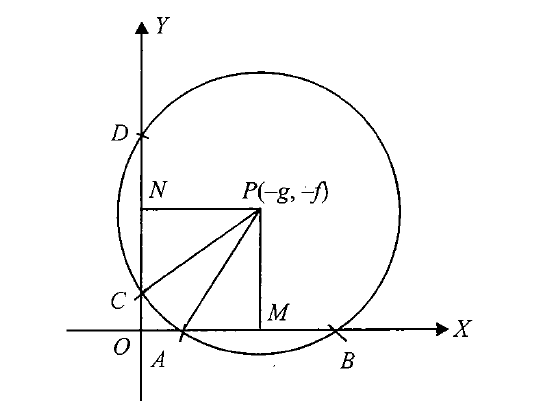
\includegraphics[scale=0.5]{circle_interecpt_on_axes.png}
    \caption{Intercept made by Circle on Axes}
\end{figure}
From diagram it is clear that,
\begin{align*}
    PM=|g|\\
    PN=|f|\\
    AP=CP=r=\sqrt{g^2+f^2-c}
\end{align*}
From triangles $CPN$ and $APM$ we have intercept terms as,
\begin{align*}
    AB=2AM=2\sqrt{f^2-c}\\
    CD=2CN=2\sqrt{g^2-c}
\end{align*}
Thing to note is that make a clear diagram of scenario that is under consideration and proceed from there.
\paragraph{\textbf{NOTE:}}
\begin{enumerate}
    \item Since intercepts are square roots, they are always positive.
    \item When circle touches either axis, then that axis has intercept to be zero since $f^2=c$ or $g^2=c$.
    \item When circle touches both axis then both intercepts are zero since $f^2=c$ and $g^2=c$.
\end{enumerate}
\end{document}